
\section{Methodology}
\label{sec:methods}


\def\ue{\ensuremath{\vec{\tilde{u}}\earth}}


% The orientation matrix can be used to rotate all vector-quantities measured in the instrument frame (velocity, rotation rate, acceleration, etc.) into the earth's coordinate system. 
% The angular rate and linear acceleration signals can be used to estimate the ADV head-motion, $\uhead$, which can then be removed from the measured velocity, $\umeas$, to estimate the `motion corrected' velocity in the earth frame,
% Note that $\uhead$ is added to $\umeas$ because the measured velocity resulting from head motion is in the opposite direction of head motion itself (i.e., $\umeas = \ue - \uhead$).

The essential approach of motion correction is to estimate the time series of velocity on a compliant mooring by obtaining an independent estimate of ADV head motion and removing that motion from the measured signal. Previous works have utilized inertial motion sensors to quantify the motion of multiscale profilers for the purpose of measuring the full spectrum of oceanic shear \cite[]{Winkel++1996}. Nortek's ADV IMU measures the linear acceleration, $\Accel$, rotational motion, $\AngRt$, and orientation matrix, $\omat$, of the ADV pressure case (body) in the Earth reference frame. So long as the ADV head is rigidly connected to the ADV pressure case, it is possible to utilize the IMU motion signals to calculate the motion of the ADV head and remove it from the measured velocity signal \cite[]{Miller++2008}. The ADV head motion is calculated as the sum of rotational and translational motion:
\begin{align}
  \label{eqn:uhead}
\begin{split}
  \uhead & = \urot + \uacc + \ulow \\
      & = \omatinv \cdot \AngRt^*(t)\times\l + \int \{\Accel(t)\}_{HP(f_{a})} \mathrm{d}t + \ulow
\end{split}
\end{align}
Here, $*$ superscripts denote quantities in the ADV's local coordinate system, and $\l$ is the vector from the IMU to the ADV head. $\omatinv$---the inverse of the orientation matrix---rotates vectors from the IMU to the Earth reference frame. The notation $\{\Accel\}_{HP(f_a)}$ indicates that the IMU's accelerometer signal is high-pass filtered (in the Earth's stationary reference frame) at a chosen filter-frequency, $f_a$. This is necessary because accelerometers have low-frequency noise, sometimes referred to as bias drift \cite[]{Barshan+Whyte1995, Bevly2004, Gulmammadov2009}.

Integrating $\Accel$ to estimate $\uacc$ amplifies the bias-drift noise at low frequencies, which dramatically reduces the signal-to-noise ratio at those time scales (Figure \ref{fig:stationary_noise}).  The high-pass filtering reduces this noise so that it does not contaminate motion correction, but real motion that exists at these frequencies is still lost in the low signal-to-noise ratio \cite[]{EgelandPhD2014, VanZwieten++2015}. This means that low-frequency motion is not well resolved by the IMU, and so there is a residual low-frequency translational motion, $\ulow$, that needs to be measured independently---or at the very least considered---when using motion-corrected ADV-IMU data. The $\AngRt$ and $\urot$ estimates do not have the same issue because there is no integration involved, and because low-frequency bias drift in the $\AngRt$ sensors is stabilized by the IMU's on-board Kalman filtering (i.e., the accelerometer and magnetometer signals provide estimates of down and north, respectively, which stabilize orientation estimates and eliminates bias from rotation estimates).

The choice of a high-pass filter for reducing low-frequency accelerometer noise depends on the flow conditions of the measurement and the platform being used. In particular, filter selection involves a trade-off between filtering out the bias-drift noise while not filtering out measured motion that is unresolved by an independent measurement of $\ulow$. If an independent measure of low-frequency motion is available it can be used to increase the accuracy of $\uhead$ at low frequency. Note that, to avoid double counting, $\ulow$ should be estimated by applying the complementary low-pass filter to the independent measurement of low-frequency motion.

With this estimate of ADV head motion, it makes sense to correct the measured velocity, $\umeas$, to estimate the velocity in the Earth's inertial reference frame:
\begin{align}
  \label{eqn:u_mot_def}
  \ue(t) & = \umeas(t) + \uhead(t).
\end{align}
Note here that the `+'-sign is correct because head motion, $\uhead$, induces a measured velocity in the opposite direction of the head motion itself ($\umeas = \ue - \uhead$).

For the TTM and Turbulence Torpedo, we utilize $f_a = 0.0333 Hz$ (30-s period) and assume that $\ulow = 0$. For the StableMoor buoy, $f_a = 0.2 Hz$ (5-s
period). The bottom-track velocity was low-pass filtered at this frequency to provide an estimate of $\ulow$, and $\Accel$ was high-pass filtered at this frequency. We use 4-pole, bidirectional (zero-phase), Hanning filters for all filtering operations. 
% * <sheri> 2016-10-21T00:00:00.000Z:
%
% Should "Turbulence Torpedo" be capitalized? Earlier it's not. If it's a product name, then yes. Otherwise, if it's a general term, then no. Please make sure you are consistent in your capitalization throughout.
%
% ^.


% Do I need to say something about filtering out gravity here too?

% Therefore, in order to remove bias-drifts in $\vec{a}$ that--when integrated according to \eqref{eqn:uacc-def}--lead to large errors in $\uacc$ this document recommends using $f_a = 0.033$Hz (30seconds). 
% On the other hand, real motions at and below $f_a$ will not be accurately accounted for in $\uacc$, and will therefore persist as low-frequency motion contamination not corrected-for in the estimate of $\vec{u}$. 

% For moorings whose low-frequency motion is limited by the mooring line itself this is a reasonable approach.  
% Assuming that the displacement of the ADV head (from the mooring's neutral position) is likely to be  $< 20 \% $ of its distance from the bottom, then for ADVs deployed at 10m depth the speed of their low-frequency motion (i.e. below $ f_a = 0.03 $ Hz) will be $<0.07 \mathrm{m/s} $.  In other words, for a 10m mooring the choice of $f_a = 0.03$Hz allows for low-frequency motion contamination on the order of 7cm/s to persist.  This is a notable but relatively minor level of uncertainty in the context of the highly energetic flows that exist at tidal energy sites.

\begin{figure}
  \centering
  \label{fig:stationary_noise}
  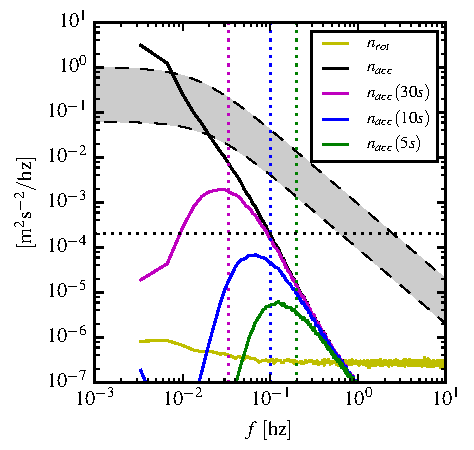
\includegraphics[width=\onewidth]{stationary_noise03}
  \caption{Spectra of $\urot$ (yellow) and $\uacc$ signals from the Microstrain IMU sitting on a motionless table. The $\uacc$ signals are unfiltered (black), and high-pass filtered at 30s (magenta), 10s (blue), 5s (green). Vertical dotted lines indicate the filter frequency. The black horizontal dotted line indicates the noise-level of a Nortek Vector ADV configured to measure $\pm$4m/s. The shaded region indicates the range of spectra presented herein (0.002 $< \tke <$ 0.03 $\mathrm{m^2/s^2}$, 1e-5 $< \epsilon <$ 5e-4 $\mathrm{W/kg}$).}
\end{figure}

Additional details on motion correction---including a detailed accounting of the distinct coordinate systems of the IMU, ADV pressure case, and ADV head---can be found in \cite{Kilcher++2016}. Open-source Python tools for performing motion correction of ADV-IMU data---including scripts that write processed data in Matlab and tabulated formats---are available at \url{http://lkilcher.github.io/dolfyn/}.

\def\ue{\ensuremath{\vec{u}\earth}}

%%% Local Variables:
%%% mode: latex
%%% TeX-master: "Kilcher_etal_IMU-ADV"
%%% End:
